
\documentclass[tikz]{standalone}

\begin{document}
\tikzset{man/.pic={
    \node[circle,fill,minimum size=5mm] (head) {};
    \node[rounded corners=2pt,minimum height=.8cm,minimum width=0.4cm,fill,below = 1pt of head] (body) {};
    \draw[line width=1mm,round cap-round cap] ([shift={(2pt,-1pt)}]body.north east) --++(-90:6mm);
    \draw[line width=1mm,round cap-round cap] ([shift={(-2pt,-1pt)}]body.north west)--++(-90:6mm);
    }}
\begin{tikzpicture}
    % one
    \node[cloud,
    draw =solarizedBase03,
    text=solarizedBase03,
    minimum width = 1mm,
    minimum height = 1mm,
    inner sep=1mm] (c) at (-.5, 0) {\tiny{$2$}};
    \pic[solarizedGreen1] at (.5, -.5) (myman) {man};
    \node[align=center] (0) at (3, 0) {
\includegraphics[width=.3\textwidth]{static/one_bit_ev}};

    \coordinate  (A) at (.5, 0);
    \coordinate  (B) at (1.5, .5) ;
    \draw [->, solarizedOrange, thicko] (A.north) to [out=90,in=180] (B.north);
    % two
    \node[cloud,
    draw =solarizedBase03,
    text=solarizedBase03,
    minimum width = 1mm,
    minimum height = 1mm,
    inner sep=1mm] (c) at (-.5, -3.5) {\tiny{$4$}};
    \pic[solarizedGreen] at (.5, -3.5) (myman) {man};
    \node[align=center] (0) at (3, -3) {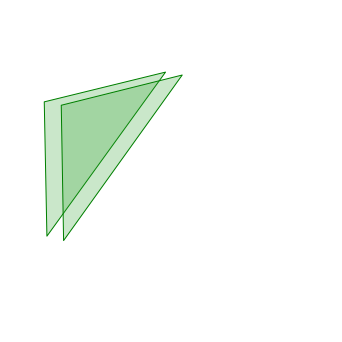
\includegraphics[width=.3\textwidth]{static/two_bit_ev}};

    \coordinate  (A) at (.5, -3);
    \coordinate  (B) at (1.5, -2.5) ;
    \draw [->, solarizedOrange, thicko] (A.north) to [out=90,in=180] (B.north);
    % three
    \node[cloud,
    draw =solarizedBase03,
    text=solarizedBase03,
    minimum width = 1mm,
    minimum height = 1mm,
    inner sep=1mm] (c) at (-.5, -6.5) {\tiny{$8$}};
    \pic[solarizedGreen2] at (.5, -6.5) (myman) {man};
    \node[align=center] (0) at (3, -6) {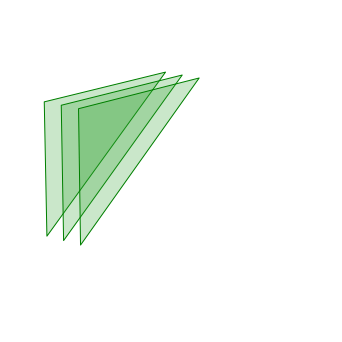
\includegraphics[width=.3\textwidth]{static/three_bit_ev}};

    \coordinate  (A) at (.5, -6);
    \coordinate  (B) at (1.5, -5.5) ;
    \draw [->, solarizedOrange, thicko] (A.north) to [out=90,in=180] (B.north);
\end{tikzpicture}
\end{document}